\documentclass[crop,tikz,border=1px]{standalone}

\usetikzlibrary{arrows,positioning,scopes,automata}

\begin{document}
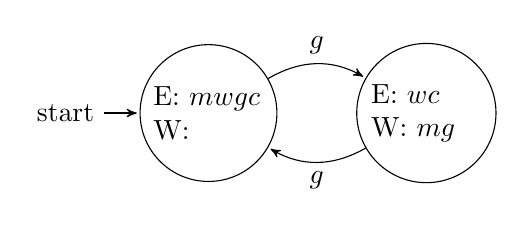
\begin{tikzpicture}[->,>=stealth',shorten >=1pt,auto,
  mystate/.style={state,inner sep=2pt,text width=1.4cm}]

  \node[initial, mystate] (s0) {E: \(mwgc\)\\W:};
  \node[mystate] (s1) [right=of s0] {E: \(wc\)\\W: \(mg\)};

  \path (s0) edge [bend left] node [above] {\(g\)} (s1)
        (s1) edge [bend left] node [below] {\(g\)} (s0);

\end{tikzpicture}
\end{document}
